\documentclass[11pt]{article}

\usepackage[margin=1in]{geometry}
\usepackage{amsmath, amssymb, mathtools}
\usepackage{graphicx}
\usepackage{booktabs}
\usepackage{tikz}
\usetikzlibrary{positioning}
\usepackage{hyperref}
\usepackage{listings}
\usepackage{verbatim}
\usepackage[T1]{fontenc}

\hypersetup{
  colorlinks=true,
  linkcolor=blue,
  citecolor=blue,
  urlcolor=blue
}

\graphicspath{{figures_bp_ar1/}}

\lstset{
  basicstyle=\ttfamily\scriptsize,
  breaklines=true,
  columns=fullflexible,
  frame=single,
  showstringspaces=false,
  keepspaces=true,
  language=Python
}

\newcommand{\R}{\mathbb{R}}
\newcommand{\E}{\mathbb{E}}
\newcommand{\N}{\mathcal{N}}
\newcommand{\dd}{\,\mathrm{d}}
\newcommand{\Cov}{\operatorname{Cov}}
\newcommand{\diag}{\operatorname{diag}}
\newcommand{\given}{\,|\,}

\title{Belief Propagation for the Gaussian AR(1) Diffusion Model\\
\large A complete derivation and numerical comparison with the precision-matrix score}
\author{Prepared for discussion with Jerome}
\date{\today}

\begin{document}
\maketitle

\begin{abstract}
This note derives belief propagation (BP) for a scalar Gaussian AR(1) clean chain observed through Ornstein-Uhlenbeck (OU) diffusion noise. The goal is to compute the diffusion score
\[
  s(x,t)=\nabla_x \log p_t(x).
\]
There are two equivalent routes. The first route uses Gaussian linear algebra: since the noisy vector is Gaussian, the score is
\[
  s(x,t)=-\Sigma_t^{-1}x.
\]
The second route uses BP on the latent AR(1) chain to compute the posterior marginals
\[
  p_t(a_i\given x_{1:n})
\]
and then the posterior means
\[
  m_i(x,t)=\E[a_i\given x_{1:n}].
\]
The score is then obtained from
\[
  s_i(x,t)=-\frac{x_i-\alpha_t m_i(x,t)}{\Delta_t}.
\]
The accompanying Python script and notebook implement both routes and verify numerically that they agree up to floating-point precision.
\end{abstract}

\tableofcontents

\section{The model}

We consider a one-dimensional sequence of clean latent variables
\[
  a_{1:n}=(a_1,\ldots,a_n)\in\R^n.
\]
The clean sequence follows a stationary Gaussian AR(1) model:
\begin{align}
  a_1 &\sim \N(0,1), \\
  a_i \given a_{i-1} &\sim \N(\rho a_{i-1},1-\rho^2), \qquad i=2,\ldots,n,
\end{align}
where
\[
  |\rho|<1.
\]
It is useful to define
\[
  q := 1-\rho^2.
\]
Then the transition can also be written as
\begin{equation}
  a_i = \rho a_{i-1}+\sqrt{q}\,\xi_i,
  \qquad \xi_i\sim \N(0,1).
\end{equation}
The choice
\[
  q=1-\rho^2
\]
keeps the marginal variance equal to one. Indeed, if \(\operatorname{Var}(a_{i-1})=1\), then
\begin{align}
  \operatorname{Var}(a_i)
  &= \operatorname{Var}(\rho a_{i-1}+\sqrt q\,\xi_i) \\
  &= \rho^2\operatorname{Var}(a_{i-1}) + q\operatorname{Var}(\xi_i) \\
  &= \rho^2 + q \\
  &= \rho^2 + (1-\rho^2) \\
  &= 1.
\end{align}
Therefore the chain is stationary with
\[
  a_i\sim \N(0,1)
\]
for every \(i\). The covariance is
\begin{equation}
  \Cov(a_i,a_j)=\rho^{|i-j|}.
\end{equation}
Thus the clean covariance matrix is
\begin{equation}
  \Sigma_0(i,j)=\rho^{|i-j|}, \qquad 1\le i,j\le n.
\end{equation}

\subsection{OU noising}

At diffusion time \(t>0\), we observe the noisy vector
\begin{equation}
  x_i = \alpha_t a_i + \sqrt{\Delta_t}\,z_i,
  \qquad z_i\sim \N(0,1),
\end{equation}
independently over \(i\), with
\begin{equation}
  \alpha_t=e^{-t},
  \qquad
  \Delta_t=1-e^{-2t}=1-\alpha_t^2.
\end{equation}
This is the standard OU corruption used in the diffusion setup. The likelihood factor for coordinate \(i\) is
\begin{equation}
  p_t(x_i\given a_i)=\N(x_i;\alpha_t a_i,\Delta_t).
\end{equation}
Since the noise variables \(z_i\) are independent, the full likelihood factorizes as
\begin{equation}
  p_t(x_{1:n}\given a_{1:n})
  =\prod_{i=1}^n \N(x_i;\alpha_t a_i,\Delta_t).
\end{equation}

\section{Posterior factorization}

The posterior distribution of the clean variables given the noisy observation is
\begin{equation}
  p_t(a_{1:n}\given x_{1:n})
  = \frac{p_0(a_{1:n})p_t(x_{1:n}\given a_{1:n})}{p_t(x_{1:n})}.
\end{equation}
Since the denominator does not depend on \(a_{1:n}\), we can write
\begin{equation}
  p_t(a_{1:n}\given x_{1:n})
  \propto
  p_0(a_{1:n})p_t(x_{1:n}\given a_{1:n}).
\end{equation}
The AR(1) prior factorizes as
\begin{equation}
  p_0(a_{1:n})
  =p(a_1)\prod_{i=2}^n p(a_i\given a_{i-1}).
\end{equation}
Therefore
\begin{equation}
  p_t(a_{1:n}\given x_{1:n})
  \propto
  p(a_1)
  \prod_{i=2}^n p(a_i\given a_{i-1})
  \prod_{i=1}^n p_t(x_i\given a_i).
\end{equation}
Define the factors
\begin{align}
  \phi_1(a_1) &:= p(a_1)=\N(a_1;0,1), \\
  \psi_i(a_{i-1},a_i) &:= p(a_i\given a_{i-1})
  =\N(a_i;\rho a_{i-1},q), \qquad i=2,\ldots,n, \\
  \ell_i(a_i;x_i) &:= p_t(x_i\given a_i)=\N(x_i;\alpha_t a_i,\Delta_t),
  \qquad i=1,\ldots,n.
\end{align}
Then the posterior becomes
\begin{equation}
  p_t(a_{1:n}\given x_{1:n})
  =\frac{1}{Z_t(x)}
  \phi_1(a_1)
  \left[\prod_{i=2}^n \psi_i(a_{i-1},a_i)\right]
  \left[\prod_{i=1}^n \ell_i(a_i;x_i)\right],
  \label{eq:posterior-factorization}
\end{equation}
where
\begin{equation}
  Z_t(x)=p_t(x_{1:n})
\end{equation}
is the evidence, also called the partition function in statistical physics language.

\section{The factor graph}

The factor graph is bipartite: variables connect to factors, and factors connect to variables. There are no factor-to-factor edges.

Formally, let
\begin{equation}
  \mathcal G=(\mathcal V,\mathcal F,\mathcal E).
\end{equation}
The variable nodes are
\begin{equation}
  \mathcal V=\{a_1,\ldots,a_n\}.
\end{equation}
The factor nodes are
\begin{equation}
  \mathcal F
  =\{\phi_1\}\cup\{\ell_1,\ldots,\ell_n\}\cup\{\psi_2,\ldots,\psi_n\}.
\end{equation}
Their scopes are
\begin{align}
  \partial \phi_1 &= \{a_1\}, \\
  \partial \ell_i &= \{a_i\}, \qquad i=1,\ldots,n, \\
  \partial \psi_i &= \{a_{i-1},a_i\}, \qquad i=2,\ldots,n.
\end{align}
Equivalently, the edge set is
\begin{equation}
\begin{aligned}
  \mathcal E
  ={}&\{(\phi_1,a_1)\}
  \cup \{(\ell_i,a_i):i=1,\ldots,n\} \\
  &\cup \{(\psi_i,a_{i-1}),(\psi_i,a_i):i=2,\ldots,n\}.
\end{aligned}
\end{equation}
Thus
\begin{equation}
  \ell_i \not\sim \psi_i.
\end{equation}
This is because \(\ell_i\) and \(\psi_i\) are both factors, and the graph is bipartite.

\begin{figure}[h!]
\centering
\begin{tikzpicture}[
  var/.style={circle,draw,minimum size=8mm,inner sep=1pt},
  factor/.style={rectangle,draw,minimum size=7mm,inner sep=1pt},
  node distance=12mm
]
  \node[var] (a1) {$a_1$};
  \node[factor,right=of a1] (p2) {$\psi_2$};
  \node[var,right=of p2] (a2) {$a_2$};
  \node[factor,right=of a2] (p3) {$\psi_3$};
  \node[var,right=of p3] (a3) {$a_3$};
  \node[right=10mm of a3] (dots) {$\cdots$};
  \node[factor,right=10mm of dots] (pn) {$\psi_n$};
  \node[var,right=of pn] (an) {$a_n$};

  \node[factor,above=of a1] (l1) {$\ell_1$};
  \node[factor,above=of a2] (l2) {$\ell_2$};
  \node[factor,above=of a3] (l3) {$\ell_3$};
  \node[factor,above=of an] (ln) {$\ell_n$};
  \node[factor,below=of a1] (phi) {$\phi_1$};

  \draw (a1)--(p2)--(a2)--(p3)--(a3);
  \draw (a3)--(dots)--(pn)--(an);
  \draw (l1)--(a1);
  \draw (l2)--(a2);
  \draw (l3)--(a3);
  \draw (ln)--(an);
  \draw (phi)--(a1);
\end{tikzpicture}
\caption{Correct factor graph for the AR(1) posterior. Each likelihood factor \(\ell_i\) attaches only to variable \(a_i\). Each transition factor \(\psi_i\) attaches to \(a_{i-1}\) and \(a_i\).}
\end{figure}

For an interior node \(a_i\), with \(2\le i\le n-1\), the neighborhood is
\begin{equation}
  \partial a_i=\{\ell_i,\psi_i,\psi_{i+1}\}.
\end{equation}
At the left boundary,
\begin{equation}
  \partial a_1=\{\phi_1,\ell_1,\psi_2\},
\end{equation}
and at the right boundary,
\begin{equation}
  \partial a_n=\{\ell_n,\psi_n\}.
\end{equation}

\section{Generic BP equations}

BP has variable-to-factor messages and factor-to-variable messages.

A variable-to-factor message is
\begin{equation}
  m_{a_i\to f}(a_i).
\end{equation}
A factor-to-variable message is
\begin{equation}
  m_{f\to a_i}(a_i).
\end{equation}
The generic BP rule from variables to factors is
\begin{equation}
  m_{a_i\to f}(a_i)
  \propto
  \prod_{g\in \partial a_i\setminus\{f\}}m_{g\to a_i}(a_i).
  \label{eq:generic-v-to-f}
\end{equation}
This means: to send a message from \(a_i\) to \(f\), multiply all incoming messages to \(a_i\), except the message coming from \(f\) itself.

The generic BP rule from factors to variables is
\begin{equation}
  m_{f\to a_i}(a_i)
  \propto
  \int
  f(a_{\partial f})
  \prod_{a_j\in\partial f\setminus\{a_i\}}
  m_{a_j\to f}(a_j)
  \prod_{a_j\in\partial f\setminus\{a_i\}}\dd a_j.
  \label{eq:generic-f-to-v}
\end{equation}
This means: to send a message from factor \(f\) to variable \(a_i\), multiply the factor by all incoming messages from the other variables in that factor, then integrate out those other variables.

For unary factors, there is no variable to integrate out. Therefore
\begin{align}
  m_{\ell_i\to a_i}(a_i)&=\ell_i(a_i;x_i), \\
  m_{\phi_1\to a_1}(a_1)&=\phi_1(a_1).
\end{align}

\section{Forward and backward messages on the chain}

Because the factor graph is a chain with unary factors attached, it is convenient to summarize messages by two directional messages.

Define \(L_i(a_i)\) as the message arriving at \(a_i\) from the left side of the graph. It contains the information from the prior and the observations to the left of site \(i\). Define \(R_i(a_i)\) as the message arriving at \(a_i\) from the right side of the graph. It contains the information from the observations to the right of site \(i\).

The boundary conditions are
\begin{equation}
  L_1(a_1)=\phi_1(a_1),
  \qquad
  R_n(a_n)=1.
\end{equation}
The forward recursion is
\begin{equation}
  L_{i+1}(a_{i+1})
  \propto
  \int
  \psi_{i+1}(a_i,a_{i+1})
  L_i(a_i)
  \ell_i(a_i;x_i)
  \dd a_i,
  \qquad i=1,\ldots,n-1.
  \label{eq:forward-density}
\end{equation}
The backward recursion is
\begin{equation}
  R_{i-1}(a_{i-1})
  \propto
  \int
  \psi_i(a_{i-1},a_i)
  R_i(a_i)
  \ell_i(a_i;x_i)
  \dd a_i,
  \qquad i=n,n-1,\ldots,2.
  \label{eq:backward-density}
\end{equation}
These equations are just the generic BP rules specialized to the chain.

\section{Beliefs and posterior marginals}

Once the left and right messages have been computed, the belief at node \(a_i\) is obtained by multiplying all information local to that node:
\begin{equation}
  b_i(a_i)
  \propto
  L_i(a_i)\ell_i(a_i;x_i)R_i(a_i).
  \label{eq:belief-propto}
\end{equation}
This is the central local rule:
\begin{equation}
  \boxed{
  \text{belief at }a_i
  =
  \text{left information}
  \times
  \text{local observation}
  \times
  \text{right information}.
  }
\end{equation}
To make \(b_i\) a probability density, normalize it:
\begin{equation}
  b_i(a_i)
  =
  \frac{L_i(a_i)\ell_i(a_i;x_i)R_i(a_i)}{
  \int L_i(u)\ell_i(u;x_i)R_i(u)\dd u}.
  \label{eq:belief-normalized}
\end{equation}
The integration variable in the denominator is written as \(u\) only to avoid confusing it with the outside variable \(a_i\).

On this tree factor graph, BP gives the exact posterior marginal:
\begin{equation}
  b_i(a_i)=p_t(a_i\given x_{1:n}).
\end{equation}
The posterior mean is
\begin{equation}
  m_i(x,t)
  :=\E[a_i\given x_{1:n}]
  =\int a_i b_i(a_i)\dd a_i.
  \label{eq:posterior-mean}
\end{equation}
This posterior mean is a Bayesian denoiser: it is the estimate of the clean latent value \(a_i\) after using the full noisy sequence \(x_{1:n}\).

\section{Why the posterior mean gives the diffusion score}

The noisy marginal is
\begin{equation}
  p_t(x_{1:n})
  =
  \int
  p_0(a_{1:n})
  \prod_{j=1}^n \N(x_j;\alpha_t a_j,\Delta_t)
  \dd a_{1:n}.
  \label{eq:noisy-marginal}
\end{equation}
The score component is
\begin{equation}
  s_i(x,t)
  :=\partial_{x_i}\log p_t(x_{1:n})
  =\frac{\partial_{x_i}p_t(x_{1:n})}{p_t(x_{1:n})}.
\end{equation}
We now compute the numerator. Only the likelihood factor involving \(x_i\) depends on \(x_i\). Therefore
\begin{align}
  \partial_{x_i}p_t(x_{1:n})
  &=
  \partial_{x_i}
  \int
  p_0(a_{1:n})
  \prod_{j=1}^n \N(x_j;\alpha_t a_j,\Delta_t)
  \dd a_{1:n} \\
  &=
  \int
  p_0(a_{1:n})
  \left[\partial_{x_i}\N(x_i;\alpha_t a_i,\Delta_t)\right]
  \prod_{j\ne i}\N(x_j;\alpha_t a_j,\Delta_t)
  \dd a_{1:n}.
\end{align}
For a one-dimensional Gaussian density as a function of \(x_i\),
\begin{equation}
  \N(x_i;\alpha_t a_i,\Delta_t)
  =\frac{1}{\sqrt{2\pi\Delta_t}}
  \exp\left[-\frac{(x_i-\alpha_t a_i)^2}{2\Delta_t}\right].
\end{equation}
Differentiate it:
\begin{align}
  \partial_{x_i}\N(x_i;\alpha_t a_i,\Delta_t)
  &=
  \N(x_i;\alpha_t a_i,\Delta_t)
  \partial_{x_i}\left[-\frac{(x_i-\alpha_t a_i)^2}{2\Delta_t}\right] \\
  &=
  \N(x_i;\alpha_t a_i,\Delta_t)
  \left[-\frac{1}{2\Delta_t}\,2(x_i-\alpha_t a_i)\right] \\
  &=
  \N(x_i;\alpha_t a_i,\Delta_t)
  \left[-\frac{x_i-\alpha_t a_i}{\Delta_t}\right].
\end{align}
Substitute this derivative into the numerator:
\begin{align}
  \partial_{x_i}p_t(x_{1:n})
  &=
  \int
  p_0(a_{1:n})
  \prod_{j=1}^n\N(x_j;\alpha_t a_j,\Delta_t)
  \left[-\frac{x_i-\alpha_t a_i}{\Delta_t}\right]
  \dd a_{1:n}.
\end{align}
Divide by \(p_t(x_{1:n})\):
\begin{align}
  s_i(x,t)
  &=
  \frac{\partial_{x_i}p_t(x_{1:n})}{p_t(x_{1:n})} \\
  &=
  \int
  \frac{p_0(a_{1:n})\prod_{j=1}^n\N(x_j;\alpha_t a_j,\Delta_t)}{p_t(x_{1:n})}
  \left[-\frac{x_i-\alpha_t a_i}{\Delta_t}\right]
  \dd a_{1:n}.
\end{align}
By Bayes' rule,
\begin{equation}
  \frac{p_0(a_{1:n})\prod_{j=1}^n\N(x_j;\alpha_t a_j,\Delta_t)}{p_t(x_{1:n})}
  =p_t(a_{1:n}\given x_{1:n}).
\end{equation}
Thus
\begin{align}
  s_i(x,t)
  &=
  \int
  p_t(a_{1:n}\given x_{1:n})
  \left[-\frac{x_i-\alpha_t a_i}{\Delta_t}\right]
  \dd a_{1:n} \\
  &=
  -\frac{1}{\Delta_t}
  \left[
  x_i\int p_t(a_{1:n}\given x_{1:n})\dd a_{1:n}
  -\alpha_t\int a_i p_t(a_{1:n}\given x_{1:n})\dd a_{1:n}
  \right] \\
  &=
  -\frac{1}{\Delta_t}
  \left[x_i-\alpha_t\E[a_i\given x_{1:n}]\right].
\end{align}
Therefore
\begin{equation}
  \boxed{
  s_i(x,t)=-\frac{x_i-\alpha_t m_i(x,t)}{\Delta_t},
  \qquad
  m_i(x,t)=\E[a_i\given x_{1:n}].
  }
  \label{eq:score-from-denoiser}
\end{equation}
This is the bridge between BP and diffusion: BP computes the posterior denoiser \(m_i(x,t)\), and the denoiser gives the diffusion score.

\section{Gaussian messages in information form}

The previous BP equations are functional equations over continuous variables. In the Gaussian case, every message remains Gaussian-shaped. Therefore each message can be stored using two scalar parameters.

We write a Gaussian-shaped message as
\begin{equation}
  m(a)\propto \exp\left(-\frac12\lambda a^2+ha\right).
  \label{eq:info-form}
\end{equation}
Here
\[
  \lambda=\text{precision},
  \qquad
  h=\text{information parameter}.
\]
If the normalized Gaussian has mean \(\mu\) and variance \(v\), then
\begin{equation}
  \lambda=\frac{1}{v},
  \qquad
  h=\frac{\mu}{v}.
\end{equation}
Conversely,
\begin{equation}
  v=\frac{1}{\lambda},
  \qquad
  \mu=\frac{h}{\lambda}.
\end{equation}
To see this, expand a Gaussian:
\begin{align}
  \N(a;\mu,v)
  &\propto
  \exp\left[-\frac{(a-\mu)^2}{2v}\right] \\
  &=
  \exp\left[-\frac{a^2-2\mu a+\mu^2}{2v}\right] \\
  &=
  \exp\left[-\frac{1}{2v}a^2+\frac{\mu}{v}a-\frac{\mu^2}{2v}\right] \\
  &\propto
  \exp\left[-\frac12\left(\frac1v\right)a^2+\left(\frac{\mu}{v}\right)a\right].
\end{align}
Thus \(\lambda=1/v\) and \(h=\mu/v\).

\subsection{Multiplying messages}

Suppose
\begin{align}
  m_1(a)&\propto \exp\left(-\frac12\lambda_1a^2+h_1a\right),\\
  m_2(a)&\propto \exp\left(-\frac12\lambda_2a^2+h_2a\right).
\end{align}
Then
\begin{align}
  m_1(a)m_2(a)
  &\propto
  \exp\left(-\frac12\lambda_1a^2+h_1a\right)
  \exp\left(-\frac12\lambda_2a^2+h_2a\right) \\
  &=
  \exp\left[-\frac12(\lambda_1+\lambda_2)a^2+(h_1+h_2)a\right].
\end{align}
Therefore multiplication corresponds to addition:
\begin{equation}
  \lambda_{\text{product}}=\lambda_1+\lambda_2,
  \qquad
  h_{\text{product}}=h_1+h_2.
  \label{eq:info-addition}
\end{equation}
This is why Gaussian BP is algebraically simple.

\subsection{Likelihood in information form}

The local likelihood is
\begin{equation}
  \ell_i(a_i;x_i)
  =\N(x_i;\alpha_t a_i,\Delta_t).
\end{equation}
As a function of \(a_i\), ignore constants independent of \(a_i\):
\begin{align}
  \ell_i(a_i;x_i)
  &\propto
  \exp\left[-\frac{(x_i-\alpha_t a_i)^2}{2\Delta_t}\right].
\end{align}
Expand the square:
\begin{equation}
  (x_i-\alpha_t a_i)^2=x_i^2-2\alpha_t x_i a_i+\alpha_t^2a_i^2.
\end{equation}
Therefore
\begin{align}
  -\frac{(x_i-\alpha_t a_i)^2}{2\Delta_t}
  &=-\frac{x_i^2}{2\Delta_t}
  +\frac{\alpha_t x_i}{\Delta_t}a_i
  -\frac{\alpha_t^2}{2\Delta_t}a_i^2 \\
  &=\text{constant in }a_i
  -\frac12\left(\frac{\alpha_t^2}{\Delta_t}\right)a_i^2
  +\left(\frac{\alpha_t x_i}{\Delta_t}\right)a_i.
\end{align}
Thus
\begin{equation}
  \ell_i(a_i;x_i)
  \propto
  \exp\left[-\frac12\lambda_\ell a_i^2+h_{\ell,i}a_i\right],
\end{equation}
with
\begin{equation}
  \lambda_\ell=\frac{\alpha_t^2}{\Delta_t},
  \qquad
  h_{\ell,i}=\frac{\alpha_t x_i}{\Delta_t}.
  \label{eq:likelihood-info}
\end{equation}
The prior \(\phi_1(a_1)=\N(a_1;0,1)\) has
\begin{equation}
  \lambda_\phi=1,
  \qquad
  h_\phi=0.
\end{equation}

\section{Gaussian forward recursion}

Let \(L_i(a_i)\) have information parameters \((\lambda_i^L,h_i^L)\). The boundary condition is
\begin{equation}
  \lambda_1^L=1,
  \qquad
  h_1^L=0.
\end{equation}
At site \(i\), before sending information to the right, multiply \(L_i\) by the local likelihood \(\ell_i\). By \eqref{eq:info-addition}, the product message has
\begin{equation}
  \lambda_i^{\to}=\lambda_i^L+\lambda_\ell,
  \qquad
  h_i^{\to}=h_i^L+h_{\ell,i}.
\end{equation}
Thus
\begin{equation}
  M_i^{\to}(a_i)
  \propto
  L_i(a_i)\ell_i(a_i;x_i)
\end{equation}
is Gaussian with
\begin{equation}
  \mu_i^{\to}=\frac{h_i^{\to}}{\lambda_i^{\to}},
  \qquad
  v_i^{\to}=\frac{1}{\lambda_i^{\to}}.
\end{equation}
The AR(1) transition says
\begin{equation}
  a_{i+1}=\rho a_i+\sqrt q\,\xi_i,
  \qquad \xi_i\sim\N(0,1).
\end{equation}
If
\[
  a_i\sim\N(\mu_i^{\to},v_i^{\to}),
\]
then
\begin{align}
  \E[a_{i+1}]&=\E[\rho a_i+\sqrt q\,\xi_i]
  =\rho \E[a_i]+\sqrt q\,\E[\xi_i]
  =\rho \mu_i^{\to}, \\
  \operatorname{Var}(a_{i+1})
  &=\operatorname{Var}(\rho a_i+\sqrt q\,\xi_i) \\
  &=\rho^2\operatorname{Var}(a_i)+q\operatorname{Var}(\xi_i) \\
  &=\rho^2v_i^{\to}+q.
\end{align}
Therefore the next left message \(L_{i+1}\) has mean and variance
\begin{equation}
  \mu_{i+1}^L=\rho\mu_i^{\to},
  \qquad
  v_{i+1}^L=q+\rho^2v_i^{\to}.
\end{equation}
Convert back to information form:
\begin{align}
  \lambda_{i+1}^L
  &=\frac{1}{v_{i+1}^L}
  =\frac{1}{q+\rho^2v_i^{\to}}
  =\frac{1}{q+\rho^2/\lambda_i^{\to}}, \\
  h_{i+1}^L
  &=\lambda_{i+1}^L\mu_{i+1}^L
  =\lambda_{i+1}^L\rho\mu_i^{\to}
  =\lambda_{i+1}^L\rho\frac{h_i^{\to}}{\lambda_i^{\to}}.
\end{align}
So the forward recursion is
\begin{equation}
  \boxed{
  \lambda_{i+1}^L=\frac{1}{q+\rho^2/\lambda_i^{\to}},
  \qquad
  h_{i+1}^L=\lambda_{i+1}^L\rho\frac{h_i^{\to}}{\lambda_i^{\to}}.
  }
\end{equation}

\section{Gaussian backward recursion}

Let \(R_i(a_i)\) have information parameters \((\lambda_i^R,h_i^R)\). The boundary condition is
\begin{equation}
  \lambda_n^R=0,
  \qquad
  h_n^R=0.
\end{equation}
This represents the constant message \(R_n(a_n)=1\), since
\[
  \exp\left(-\frac12\cdot0\cdot a_n^2+0\cdot a_n\right)=1.
\]
At site \(i\), multiply \(R_i\) by the local likelihood. The product has
\begin{equation}
  \lambda_i^{\leftarrow}=\lambda_i^R+\lambda_\ell,
  \qquad
  h_i^{\leftarrow}=h_i^R+h_{\ell,i}.
\end{equation}
Thus
\begin{equation}
  M_i^{\leftarrow}(a_i)
  \propto
  R_i(a_i)\ell_i(a_i;x_i)
\end{equation}
is Gaussian with
\begin{equation}
  \mu_i^{\leftarrow}=\frac{h_i^{\leftarrow}}{\lambda_i^{\leftarrow}},
  \qquad
  v_i^{\leftarrow}=\frac{1}{\lambda_i^{\leftarrow}}.
\end{equation}
Now compute
\begin{equation}
  R_{i-1}(a_{i-1})
  \propto
  \int \N(a_i;\rho a_{i-1},q)
  M_i^{\leftarrow}(a_i)
  \dd a_i.
\end{equation}
Since
\[
  M_i^{\leftarrow}(a_i)\propto \N(a_i;\mu_i^{\leftarrow},v_i^{\leftarrow}),
\]
we need the integral
\begin{equation}
  \int
  \N(a_i;\rho a_{i-1},q)
  \N(a_i;\mu_i^{\leftarrow},v_i^{\leftarrow})
  \dd a_i.
\end{equation}
The Gaussian product identity gives
\begin{equation}
  \int \N(y;m_1,v_1)\N(y;m_2,v_2)\dd y
  =\N(m_1;m_2,v_1+v_2).
\end{equation}
Here
\[
  y=a_i,
  \qquad
  m_1=\rho a_{i-1},
  \qquad
  v_1=q,
  \qquad
  m_2=\mu_i^{\leftarrow},
  \qquad
  v_2=v_i^{\leftarrow}.
\]
Therefore
\begin{equation}
  R_{i-1}(a_{i-1})
  \propto
  \N(\mu_i^{\leftarrow};\rho a_{i-1},q+v_i^{\leftarrow}).
\end{equation}
As a function of \(a_{i-1}\), this is
\begin{align}
  R_{i-1}(a_{i-1})
  &\propto
  \exp\left[-\frac{(\mu_i^{\leftarrow}-\rho a_{i-1})^2}{2(q+v_i^{\leftarrow})}\right] \\
  &=
  \exp\left[-\frac{(\mu_i^{\leftarrow})^2-2\rho\mu_i^{\leftarrow}a_{i-1}+\rho^2a_{i-1}^2}{2(q+v_i^{\leftarrow})}\right] \\
  &\propto
  \exp\left[-\frac12\left(\frac{\rho^2}{q+v_i^{\leftarrow}}\right)a_{i-1}^2
  +\left(\frac{\rho\mu_i^{\leftarrow}}{q+v_i^{\leftarrow}}\right)a_{i-1}\right].
\end{align}
Thus
\begin{equation}
  \lambda_{i-1}^R=\frac{\rho^2}{q+v_i^{\leftarrow}},
  \qquad
  h_{i-1}^R=\frac{\rho\mu_i^{\leftarrow}}{q+v_i^{\leftarrow}}.
\end{equation}
Now substitute
\[
  v_i^{\leftarrow}=\frac1{\lambda_i^{\leftarrow}},
  \qquad
  \mu_i^{\leftarrow}=\frac{h_i^{\leftarrow}}{\lambda_i^{\leftarrow}}.
\]
For the precision:
\begin{align}
  \lambda_{i-1}^R
  &=\frac{\rho^2}{q+1/\lambda_i^{\leftarrow}} \\
  &=\frac{\rho^2}{(q\lambda_i^{\leftarrow}+1)/\lambda_i^{\leftarrow}} \\
  &=\frac{\rho^2\lambda_i^{\leftarrow}}{q\lambda_i^{\leftarrow}+1}.
\end{align}
For the information parameter:
\begin{align}
  h_{i-1}^R
  &=\frac{\rho (h_i^{\leftarrow}/\lambda_i^{\leftarrow})}{q+1/\lambda_i^{\leftarrow}} \\
  &=\frac{\rho h_i^{\leftarrow}/\lambda_i^{\leftarrow}}{(q\lambda_i^{\leftarrow}+1)/\lambda_i^{\leftarrow}} \\
  &=\frac{\rho h_i^{\leftarrow}}{q\lambda_i^{\leftarrow}+1}.
\end{align}
So the backward recursion is
\begin{equation}
  \boxed{
  \lambda_{i-1}^R=\frac{\rho^2\lambda_i^{\leftarrow}}{q\lambda_i^{\leftarrow}+1},
  \qquad
  h_{i-1}^R=\frac{\rho h_i^{\leftarrow}}{q\lambda_i^{\leftarrow}+1}.
  }
\end{equation}

\section{Final Gaussian beliefs}

The belief is
\begin{equation}
  b_i(a_i)\propto L_i(a_i)\ell_i(a_i;x_i)R_i(a_i).
\end{equation}
Since multiplication adds information parameters,
\begin{equation}
  \lambda_i^b=\lambda_i^L+\lambda_\ell+\lambda_i^R,
  \qquad
  h_i^b=h_i^L+h_{\ell,i}+h_i^R.
\end{equation}
Hence
\begin{equation}
  b_i(a_i)=\N(a_i;\mu_i^b,v_i^b),
\end{equation}
where
\begin{equation}
  v_i^b=\frac1{\lambda_i^b},
  \qquad
  \mu_i^b=\frac{h_i^b}{\lambda_i^b}.
\end{equation}
Therefore
\begin{equation}
  m_i(x,t)=\E[a_i\given x_{1:n}]=\mu_i^b.
\end{equation}
The BP score is then
\begin{equation}
  s_i^{\mathrm{BP}}(x,t)
  =-\frac{x_i-\alpha_t\mu_i^b}{\Delta_t}.
\end{equation}

\section{The precision-matrix route}

Because the model is Gaussian, the noisy vector is also Gaussian. In vector form,
\begin{equation}
  x=\alpha_t a+\sqrt{\Delta_t}\,z,
  \qquad
  a\sim\N(0,\Sigma_0),
  \qquad
  z\sim\N(0,I).
\end{equation}
Therefore
\begin{align}
  \Sigma_t
  :=\Cov(x)
  &=\Cov(\alpha_t a+\sqrt{\Delta_t}\,z) \\
  &=\alpha_t^2\Cov(a)+\Delta_t\Cov(z) \\
  &=\alpha_t^2\Sigma_0+\Delta_t I.
\end{align}
Thus
\begin{equation}
  x\sim\N(0,\Sigma_t).
\end{equation}
The log-density is
\begin{equation}
  \log p_t(x)
  =-\frac12x^\top\Sigma_t^{-1}x
  -\frac12\log\det(2\pi\Sigma_t).
\end{equation}
The second term does not depend on \(x\). Differentiating the quadratic term gives
\begin{equation}
  \nabla_x\left(-\frac12x^\top\Sigma_t^{-1}x\right)
  =-\Sigma_t^{-1}x,
\end{equation}
because \(\Sigma_t^{-1}\) is symmetric. Hence
\begin{equation}
  \boxed{
  s^{\mathrm{matrix}}(x,t)=-\Sigma_t^{-1}x.
  }
\end{equation}
The posterior mean under the Gaussian linear model is
\begin{equation}
  \E[a\given x]
  =\Cov(a,x)\Cov(x,x)^{-1}x.
\end{equation}
Now
\begin{align}
  \Cov(a,x)
  &=\Cov(a,\alpha_t a+\sqrt{\Delta_t}z) \\
  &=\alpha_t\Cov(a,a)+\sqrt{\Delta_t}\Cov(a,z) \\
  &=\alpha_t\Sigma_0,
\end{align}
since \(a\) and \(z\) are independent. Also \(\Cov(x,x)=\Sigma_t\). Therefore
\begin{equation}
  \boxed{
  \E[a\given x]=\alpha_t\Sigma_0\Sigma_t^{-1}x.
  }
\end{equation}

\section{Algebraic equivalence of the two score formulas}

Start from the BP score formula:
\begin{equation}
  s^{\mathrm{BP}}(x,t)
  =-\frac{x-\alpha_t\E[a\given x]}{\Delta_t}.
\end{equation}
Using the Gaussian posterior mean,
\begin{equation}
  \E[a\given x]=\alpha_t\Sigma_0\Sigma_t^{-1}x.
\end{equation}
Substitute this into the BP score:
\begin{align}
  s^{\mathrm{BP}}(x,t)
  &=-\frac{x-\alpha_t(\alpha_t\Sigma_0\Sigma_t^{-1}x)}{\Delta_t} \\
  &=-\frac{x-\alpha_t^2\Sigma_0\Sigma_t^{-1}x}{\Delta_t}.
\end{align}
Now use
\begin{equation}
  \Sigma_t=\alpha_t^2\Sigma_0+\Delta_t I.
\end{equation}
Rearrange it:
\begin{equation}
  \Delta_t I=\Sigma_t-\alpha_t^2\Sigma_0.
\end{equation}
Multiply both sides by \(\Sigma_t^{-1}x\):
\begin{align}
  \Delta_t I\Sigma_t^{-1}x
  &=(\Sigma_t-\alpha_t^2\Sigma_0)\Sigma_t^{-1}x \\
  \Delta_t\Sigma_t^{-1}x
  &=\Sigma_t\Sigma_t^{-1}x-\alpha_t^2\Sigma_0\Sigma_t^{-1}x \\
  \Delta_t\Sigma_t^{-1}x
  &=x-\alpha_t^2\Sigma_0\Sigma_t^{-1}x.
\end{align}
Therefore
\begin{equation}
  \frac{x-\alpha_t^2\Sigma_0\Sigma_t^{-1}x}{\Delta_t}
  =\Sigma_t^{-1}x.
\end{equation}
Substitute this into the BP score:
\begin{equation}
  s^{\mathrm{BP}}(x,t)
  =-\Sigma_t^{-1}x
  =s^{\mathrm{matrix}}(x,t).
\end{equation}
So the two algorithms must agree:
\begin{equation}
  \boxed{
  s^{\mathrm{BP}}(x,t)=s^{\mathrm{matrix}}(x,t).
  }
\end{equation}

\section{Algorithm summary}

Given \(x_{1:n}\), \(\rho\), and \(t>0\):
\begin{enumerate}
  \item Set
  \[
    \alpha_t=e^{-t},
    \qquad
    \Delta_t=1-e^{-2t},
    \qquad
    q=1-\rho^2.
  \]
  \item Set likelihood information parameters
  \[
    \lambda_\ell=\frac{\alpha_t^2}{\Delta_t},
    \qquad
    h_{\ell,i}=\frac{\alpha_t x_i}{\Delta_t}.
  \]
  \item Initialize the left messages:
  \[
    \lambda_1^L=1,
    \qquad
    h_1^L=0.
  \]
  \item For \(i=1,\ldots,n-1\), compute
  \[
    \lambda_i^{\to}=\lambda_i^L+\lambda_\ell,
    \qquad
    h_i^{\to}=h_i^L+h_{\ell,i},
  \]
  then
  \[
    \lambda_{i+1}^L=\frac{1}{q+\rho^2/\lambda_i^{\to}},
    \qquad
    h_{i+1}^L=\lambda_{i+1}^L\rho\frac{h_i^{\to}}{\lambda_i^{\to}}.
  \]
  \item Initialize the right messages:
  \[
    \lambda_n^R=0,
    \qquad
    h_n^R=0.
  \]
  \item For \(i=n,n-1,\ldots,2\), compute
  \[
    \lambda_i^{\leftarrow}=\lambda_i^R+\lambda_\ell,
    \qquad
    h_i^{\leftarrow}=h_i^R+h_{\ell,i},
  \]
  then
  \[
    \lambda_{i-1}^R=\frac{\rho^2\lambda_i^{\leftarrow}}{q\lambda_i^{\leftarrow}+1},
    \qquad
    h_{i-1}^R=\frac{\rho h_i^{\leftarrow}}{q\lambda_i^{\leftarrow}+1}.
  \]
  \item Compute the belief parameters:
  \[
    \lambda_i^b=\lambda_i^L+\lambda_\ell+\lambda_i^R,
    \qquad
    h_i^b=h_i^L+h_{\ell,i}+h_i^R.
  \]
  \item Compute the posterior mean and variance:
  \[
    \mu_i^b=\frac{h_i^b}{\lambda_i^b},
    \qquad
    v_i^b=\frac1{\lambda_i^b}.
  \]
  \item Compute the BP score:
  \[
    s_i^{\mathrm{BP}}(x,t)=-\frac{x_i-\alpha_t\mu_i^b}{\Delta_t}.
  \]
  \item Compute the matrix score for comparison:
  \[
    \Sigma_0(i,j)=\rho^{|i-j|},
    \qquad
    \Sigma_t=\alpha_t^2\Sigma_0+\Delta_t I,
  \]
  \[
    s^{\mathrm{matrix}}(x,t)=-\Sigma_t^{-1}x.
  \]
\end{enumerate}

\section{Numerical output from the accompanying script}

The Python script creates one synthetic AR(1) sample, corrupts it with OU noise, computes the score using both routes, and compares the results. With the default parameters
\[
  n=40,
  \qquad
  \rho=0.7,
  \qquad
  t=0.8,
\]
the script writes the following summary.

\verbatiminput{figures_bp_ar1/results_summary.txt}

The differences are at the level of floating-point roundoff. This is exactly what we expect from the algebraic equivalence shown above.

\section{Generated plots}

The first plot shows the clean latent sample, the noisy observation, and the posterior mean computed by both methods.

\begin{figure}[h!]
\centering
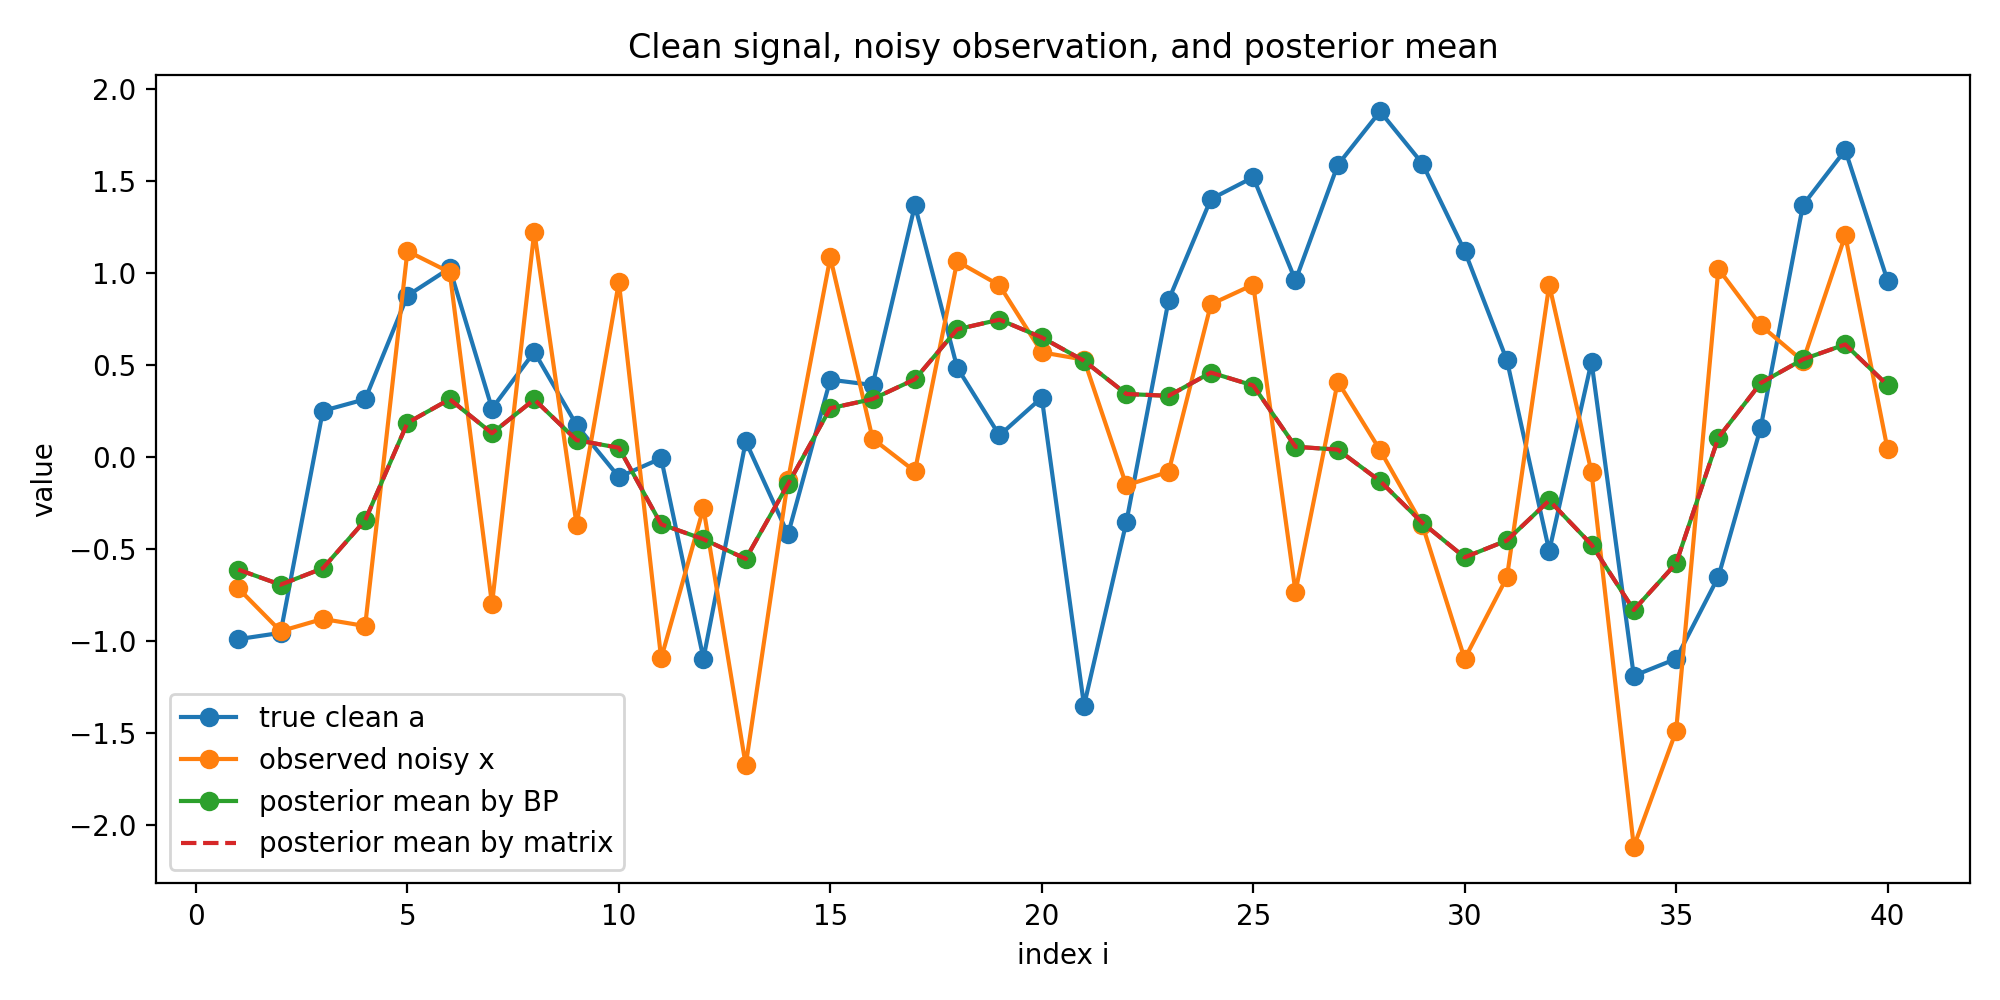
\includegraphics[width=0.92\textwidth]{clean_noisy_posterior.png}
\caption{The posterior mean is the Bayesian denoiser \(\E[a_i\given x_{1:n}]\). The BP and matrix posterior means overlap.}
\end{figure}

\begin{figure}[h!]
\centering
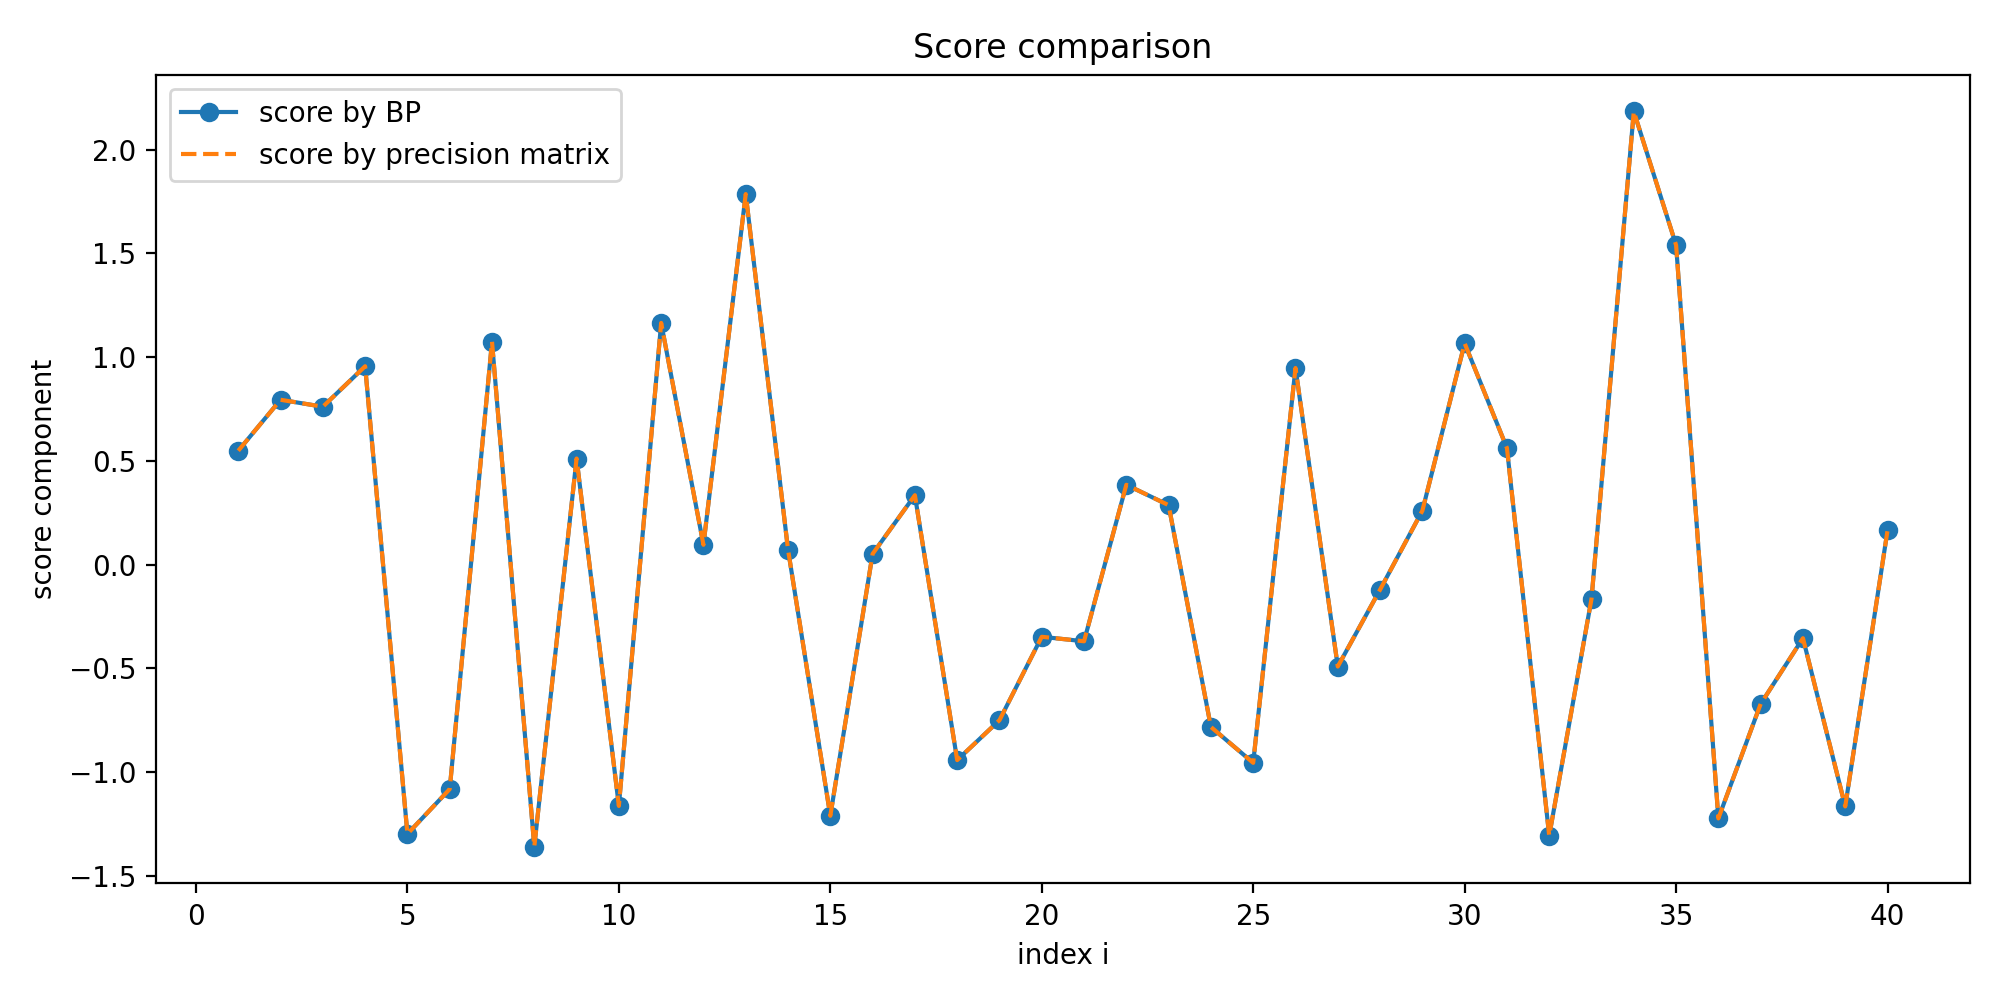
\includegraphics[width=0.92\textwidth]{score_comparison.png}
\caption{Score components computed by BP and by the precision matrix. The curves overlap.}
\end{figure}

\begin{figure}[h!]
\centering
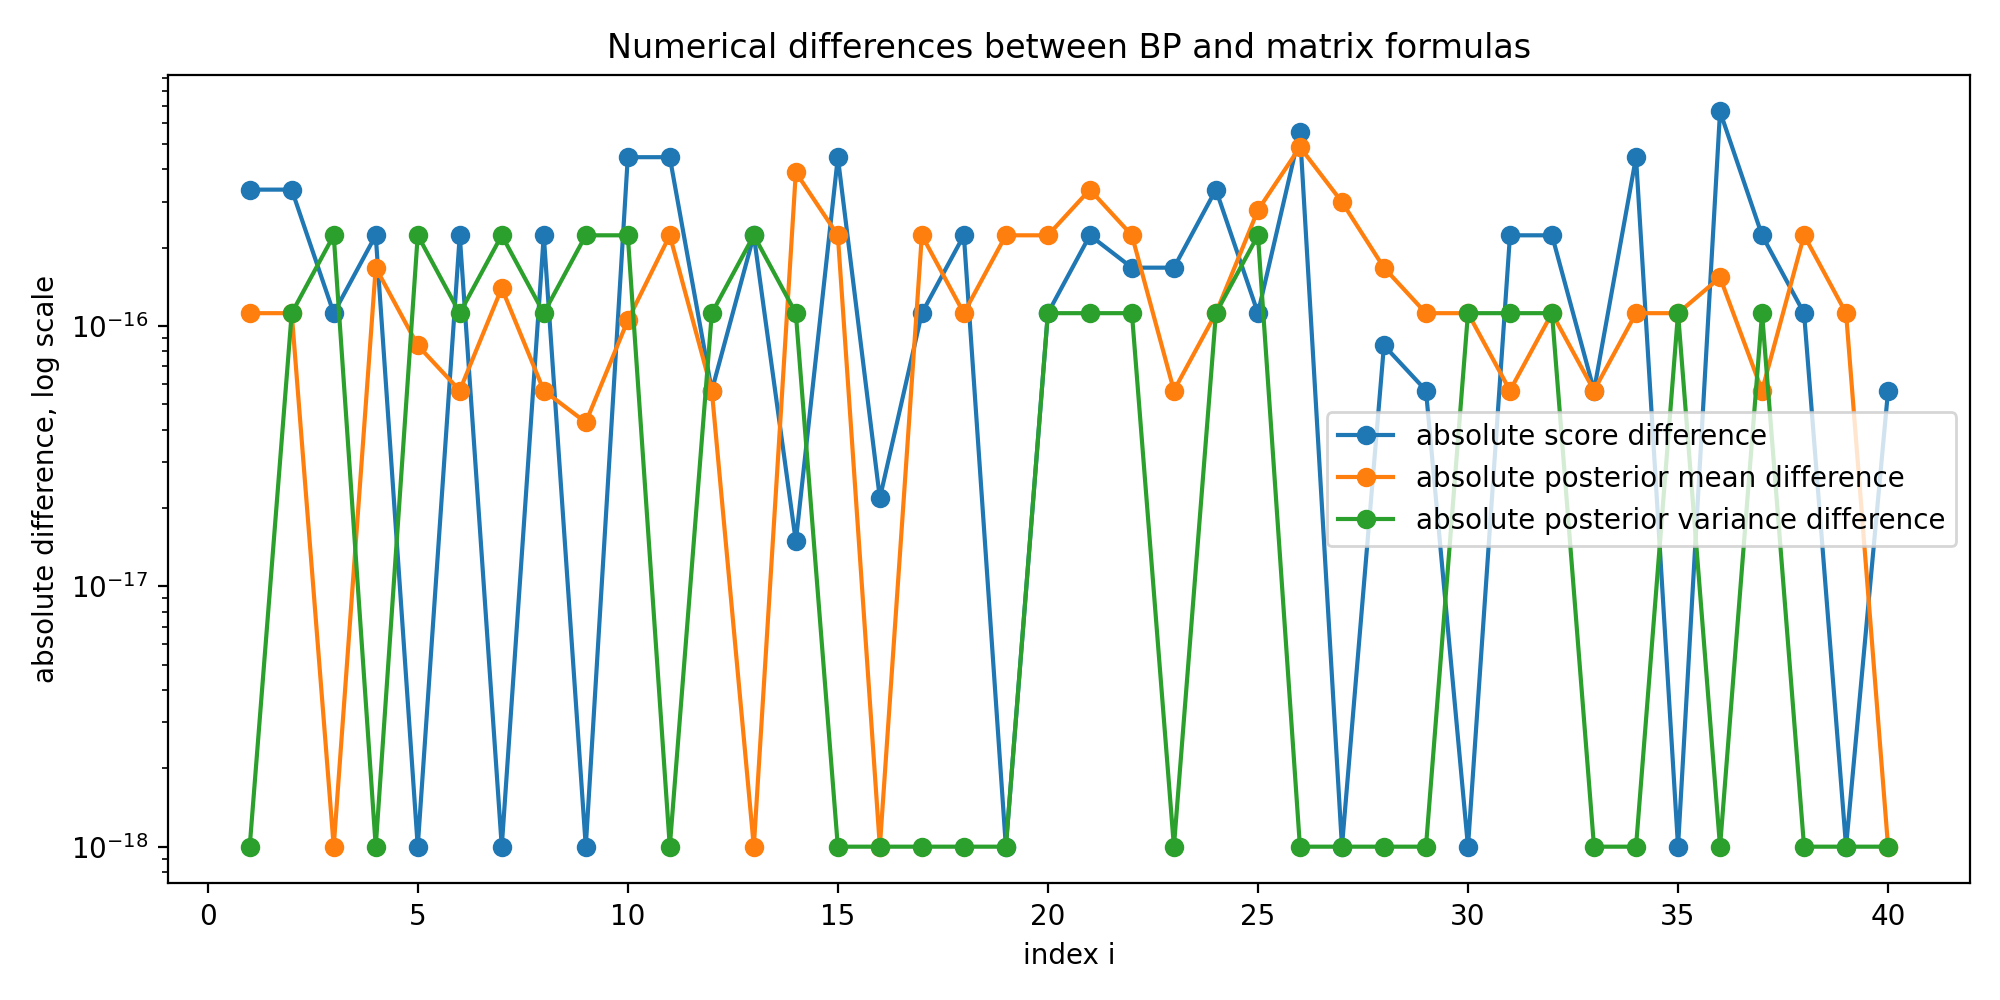
\includegraphics[width=0.92\textwidth]{absolute_differences.png}
\caption{Absolute differences between BP and matrix outputs. The scale is logarithmic.}
\end{figure}

\begin{figure}[h!]
\centering
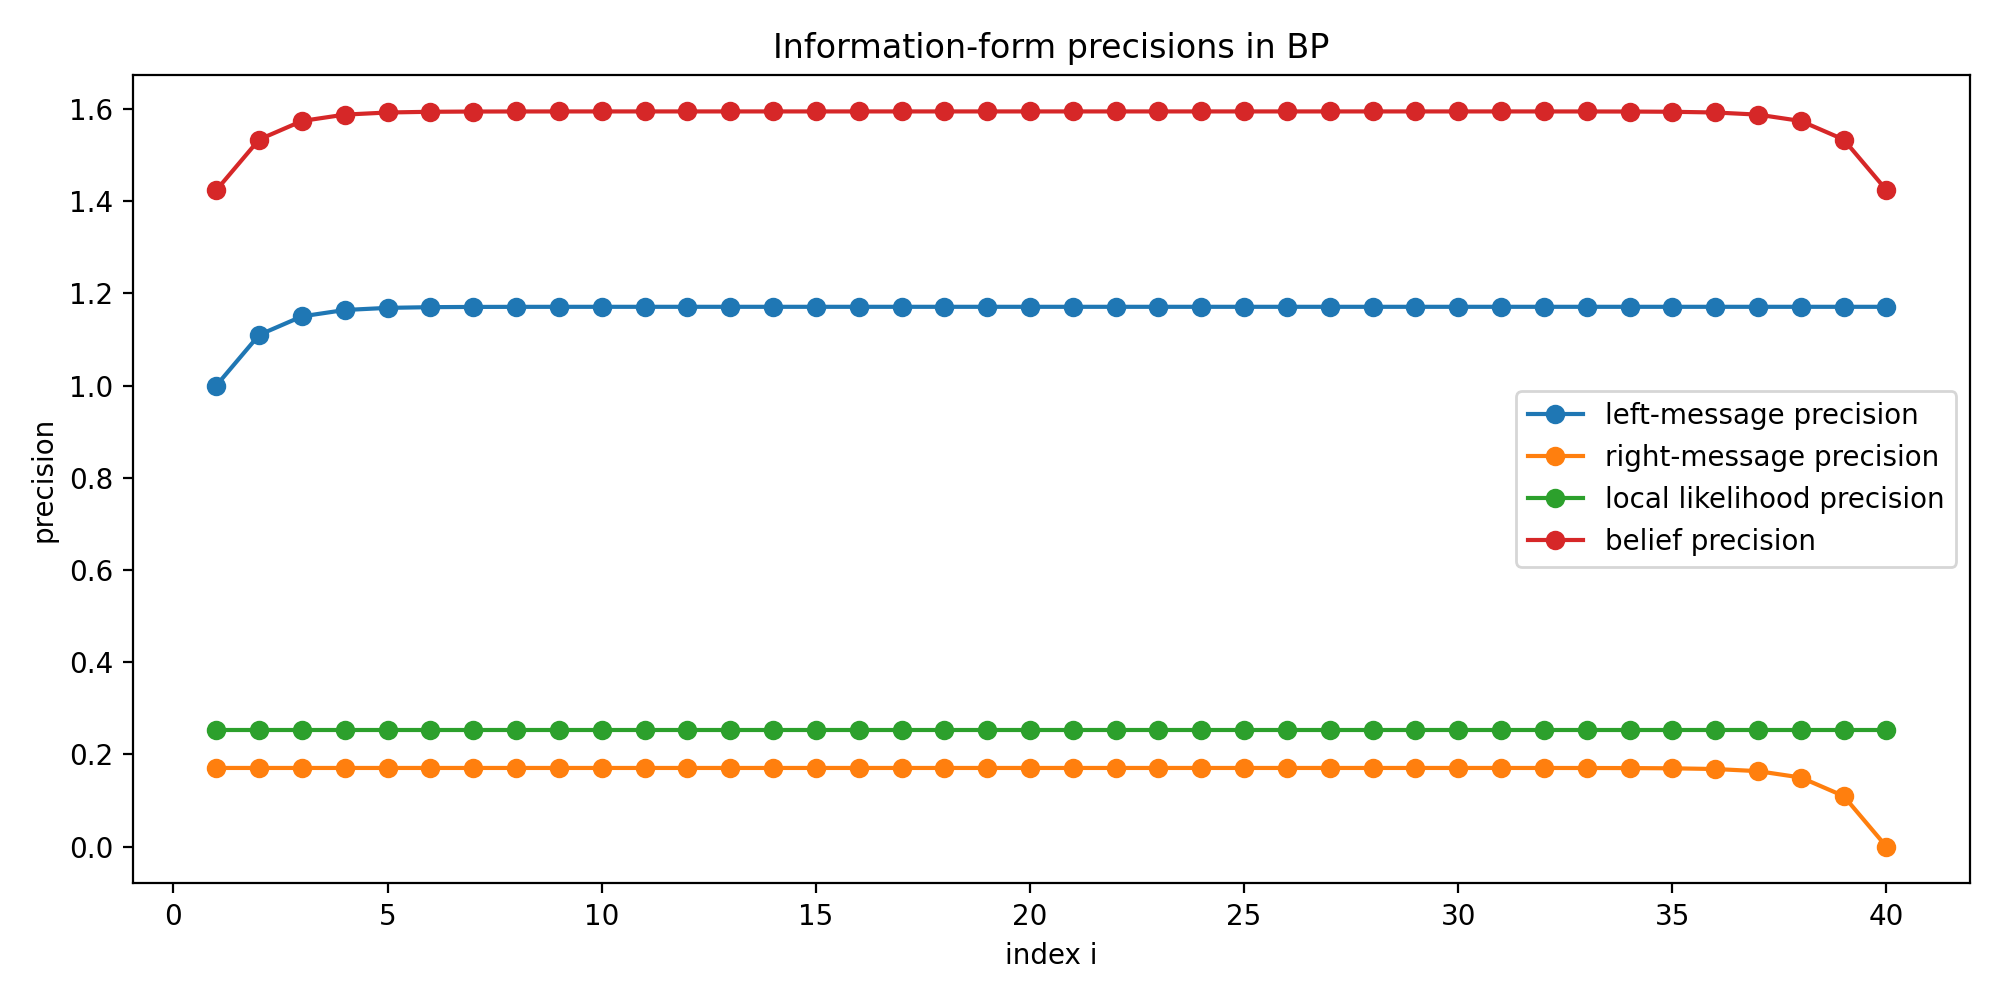
\includegraphics[width=0.92\textwidth]{bp_message_precisions.png}
\caption{Information-form precisions appearing in BP. The belief precision is the sum of left-message, local-likelihood, and right-message precisions.}
\end{figure}

\begin{figure}[h!]
\centering
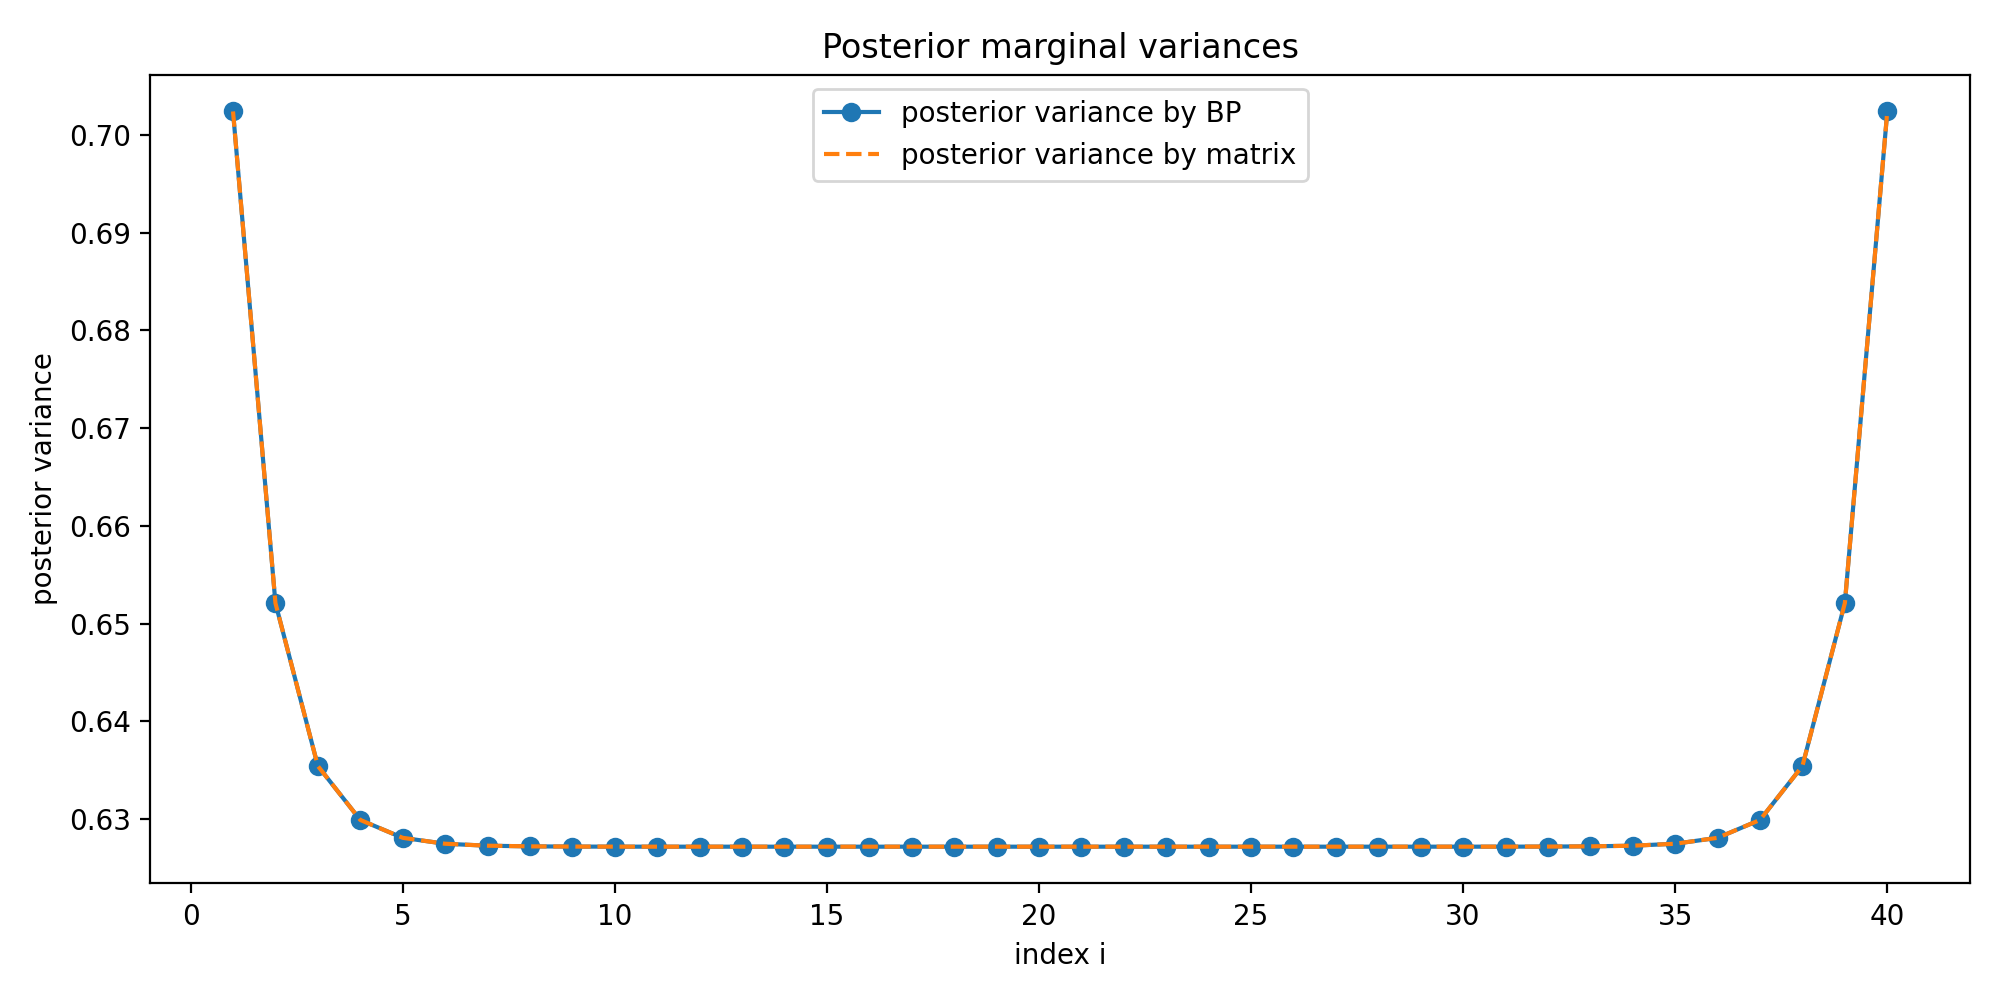
\includegraphics[width=0.92\textwidth]{posterior_variance.png}
\caption{Posterior marginal variances from BP and from the Gaussian matrix formula.}
\end{figure}

\clearpage
\section{How to use the files}

The project contains four main files:
\begin{itemize}
  \item \texttt{bp\_gaussian\_ar1\_diffusion.tex}: the LaTeX source for this document.
  \item \texttt{bp\_gaussian\_ar1\_diffusion.pdf}: the compiled PDF.
  \item \texttt{bp\_gaussian\_ar1\_diffusion.py}: a standalone Python script.
  \item \texttt{bp\_gaussian\_ar1\_diffusion.ipynb}: a notebook version for interactive experiments and plots.
\end{itemize}
To run the Python script from a terminal:
\begin{verbatim}
python bp_gaussian_ar1_diffusion.py --n 40 --rho 0.7 --t 0.8 --seed 123
\end{verbatim}
This creates a folder called \texttt{figures\_bp\_ar1} containing the plots and a text summary. You can modify \(n\), \(\rho\), \(t\), and the random seed from the command line.

\section{References and context}

The OU noising model and the identity relating the score to a posterior expectation are standard in the diffusion-model literature. In the notation used here, the identity is
\[
  \nabla_{x_i}\log p_t(x)
  =-\frac{x_i-\alpha_t\E[a_i\given x]}{\Delta_t}.
\]
The BP equations used here are the usual sum-product equations on factor graphs. In continuous variables, messages are densities; in the Gaussian case, these densities close exactly inside the Gaussian family and can be represented by precision and information parameters.

\begin{thebibliography}{9}
\bibitem{BiroliMezard2023}
G. Biroli and M. Mezard.
\newblock Generative diffusion in very large dimensions.
\newblock arXiv:2306.03518, 2023.

\bibitem{MezardNotes2025}
M. Mezard.
\newblock Generative diffusion updated notes.
\newblock Lecture notes, December 2025.

\bibitem{MezardMontanari2008}
M. Mezard and A. Montanari.
\newblock Information, Physics, and Computation.
\newblock Oxford University Press, 2009; draft chapters circulated in 2008.

\bibitem{GenovesePiana2026}
G. Genovese and A. Piana.
\newblock Derivation of the AMP equations from belief propagation for the \(\ell_2\) minimisation problem.
\newblock arXiv:2602.15191, 2026.
\end{thebibliography}

\appendix
\clearpage
\section{Full Python source code}

\lstinputlisting{bp_gaussian_ar1_diffusion.py}

\end{document}
